\subsection{Rapid Test Statistics}
\label{subsec:results_rapid_test_statistics}

An important feature in our model is that our rapid tests are imperfectly specific and
imperfectly sensitive. Especially when people have not become infectious yet rapid tests
are likely to return a false positive result. Here we look at how rapid tests expanded
over time and to what degree they are useful as a screening device despite missing
positive cases and returning false positive results.

We start with the share of the population doing a rapid test, receiving a positive rapid
test and receiving a negative rapid test over time by the channel through which the test
was demanded in Figures~\ref{fig:rapid_test_demand_by_channel},
\ref{fig:pos_rapid_tests_by_channel} and \ref{fig:neg_rapid_tests_by_channel},
respectively. Overall, the share of the population getting a rapid test on a given day
increases from 2\% in mid March to over 10\% by May. The work rapid tests are a little
ragged because of public holidays. For education rapid tests both vacations (first half
of April) as well as the opening of schools in May are very visible in the rapid test
demand. Overall, work tests make up the largest fraction of rapid tests. The image is
very similar for the share of positive tests, except that the overall number of positive
tests starts decreasing in May as rapid test expansion comes to a halt and cases fall,
especially the positive share of private rapid tests falls as less and less individuals
seek a rapid test because of a positive test in their household.

\begin{figure}[ht] % Share tested per day
  \centering
  \begin{subfigure}[b]{0.3\textwidth}
      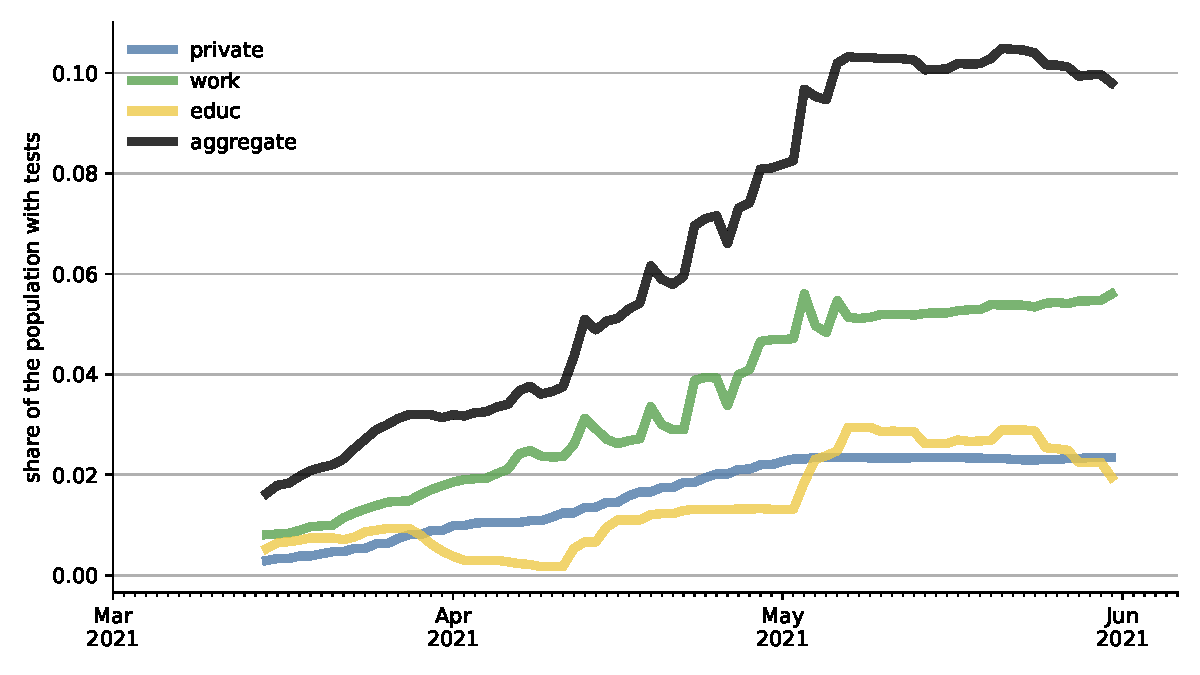
\includegraphics[width=\textwidth]{figures/results/figures/rapid_test_statistics/popshare_tested}
      \caption{Share of the Population Doing a Rapid Test Because of Different Channels
      on a Given Day}
      \label{fig:rapid_test_demand_by_channel}
  \end{subfigure}
  \hfill
  \begin{subfigure}[b]{0.3\textwidth}
      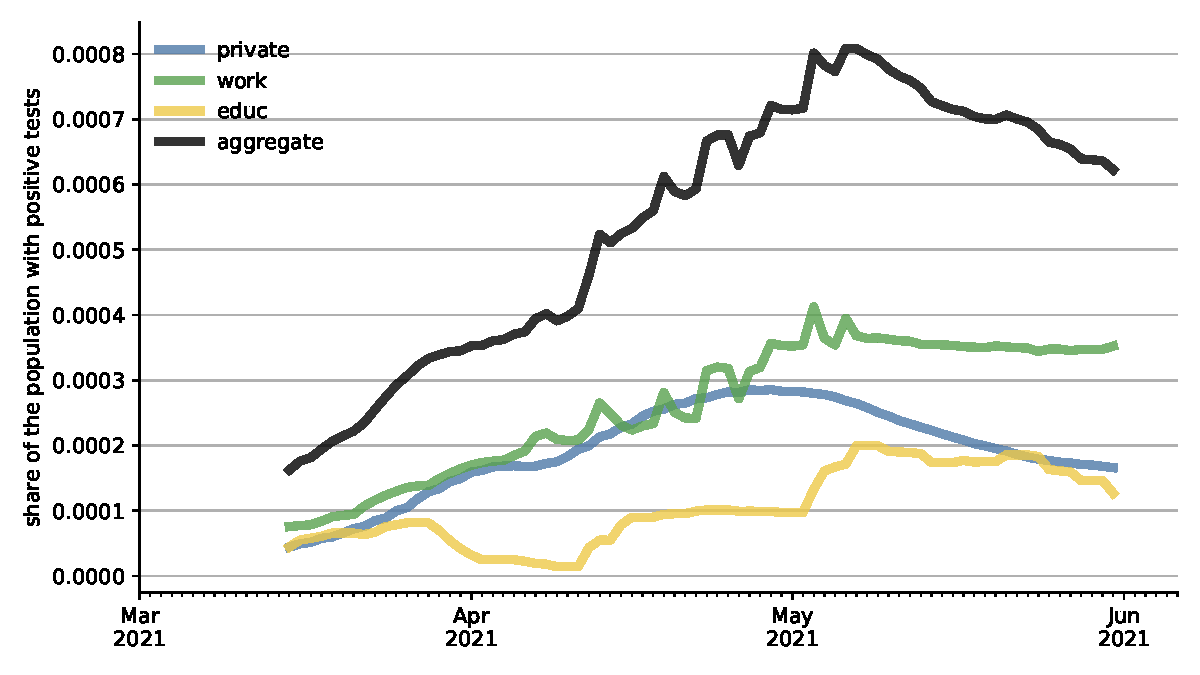
\includegraphics[width=\textwidth]{figures/results/figures/rapid_test_statistics/popshare_tested_positive}
      \caption{Share of the Population Testing Positive Because of Different Channels
      on a Given Day}
      \label{fig:pos_rapid_tests_by_channel}
  \end{subfigure}
  \hfill
  \begin{subfigure}[b]{0.3\textwidth}
      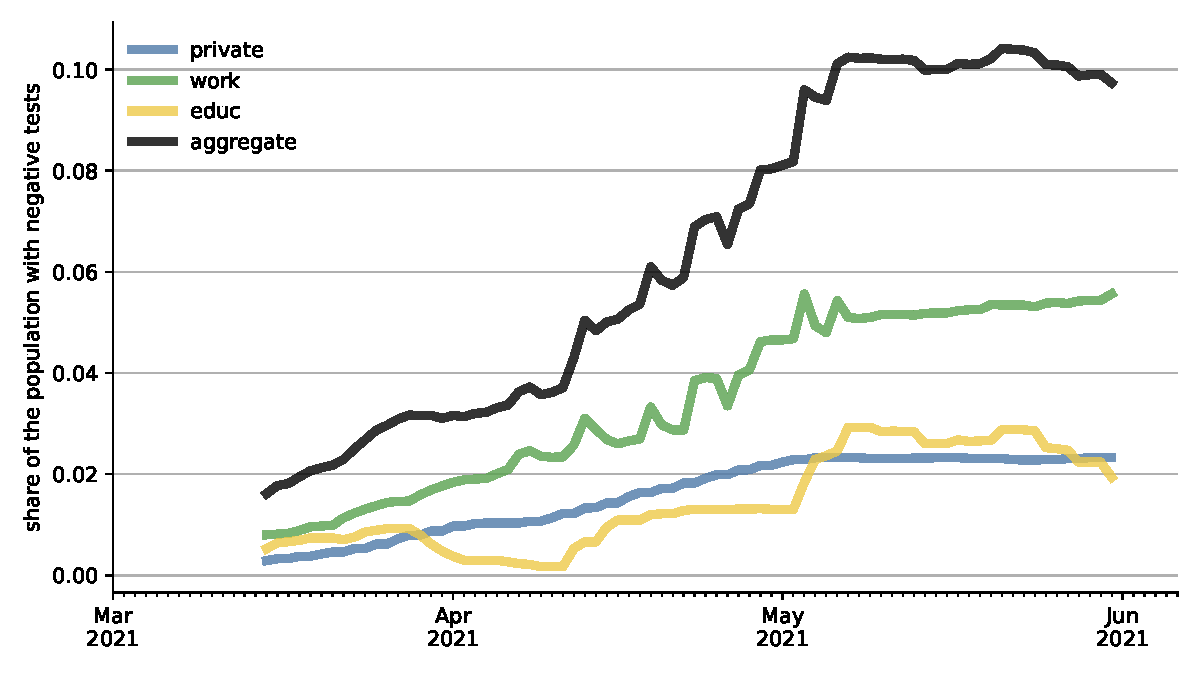
\includegraphics[width=\textwidth]{figures/results/figures/rapid_test_statistics/popshare_tested_negative}
      \caption{Share of the Population Testing Negative Because of Different Channels
      on a Given Day}
      \label{fig:neg_rapid_tests_by_channel}
  \end{subfigure}
  \caption{Rapid Test Shares in the Population by Channel}
  \floatfoot{\noindent \textit{Note:}
    Rapid tests in the education setting are demanded by teachers (nursery, preschool and
    school) as well as school pupils. After Easter the required frequency of tests is
    increased from once per week to twice per week. Work rapid tests are demanded by
    individuals that still have work contacts, i.e. do not work from home. The share of
    employers offering rapid tests increases over the time frame and the frequency of
    testing is also increased. Tests are demanded by individuals for one of three private
    reasons: having developed symptoms without access to a PCR test, having a household
    member that has tested positive or developed symptoms or having planned weekly
    meeting with friends. The left figure shows the share of the population doing a
    rapid test on a given day. The middle figure shows the share of the population
    testing positive on a given day (true and false positives). The right figure shows
    the share of the population testing negative on a given day (true and false
    negatives).}
\end{figure}

\FloatBarrier

Next, we show the tests split by whether they are true positive, false positive, true
negative or false negative (see Figure~\ref{fig:rapid_test_results_numbers}) in numbers
per million individuals to have a more legible metric.
% true positive
The number of true positives (Figure~\ref{fig:rapid_tests_number_true_positive}) rapidly
increases and peaks at the end of April with over 200 cases per million detected through
rapid tests per day. This means that our model suggests that Germany was able to detect
up to 16,600 cases per day that would have likely gone undetected otherwise. The most
powerful tool for detecting cases are the private rapid tests. This is because a large
share of them are targeted, i.e. triggered by events in the household. Thus, we have to
be careful to interpret them, as many private tests are likely to be triggered by cases
detected through work rapid tests. Thus, it's unsurprising that their Shapley value
(Figure~\ref{fig:2021_scenarios_decomposition_tests}) implies that their contribution is
only 50\% of the effect of rapid tests with work rapid tests accounting for over 40\% of
the effect of rapid tests and schools only accounting for 7\%.
% false positive and true negative
Turning to the number of false positive tests
(Figure~\ref{fig:rapid_tests_number_false_positive}) we see that the number of false
positives increases until May during which the number of actual cases declines and
testing expands, both leading to more false positive test results. The same pattern
emerges for the true negative tests (Figure~\ref{fig:rapid_tests_number_true_negative})
but on a much larger scale. Overall the number of false positives is negligible. Less
than 0.07\% of the population test false positive.
% false negative
Lastly, concerning worries about the accuracy of rapid tests, our model has very
encouraging results. Despite modeling in detail the low sensitivity of rapid tests before
the onset of infectiousness, there are very few (less than 80 cases per million per day)
false negative results as can be seen in
Figure~\ref{fig:rapid_tests_false_negative_rate}. The false negative rate is highest for
private demand because many household members perform the rapid test in response to an
infected household member because they themselves become infectious.

\begin{figure}   % Number of True Positive / False Positive / True Negative / False Negative
    \centering
    \begin{subfigure}[b]{0.425\textwidth}
        \centering
        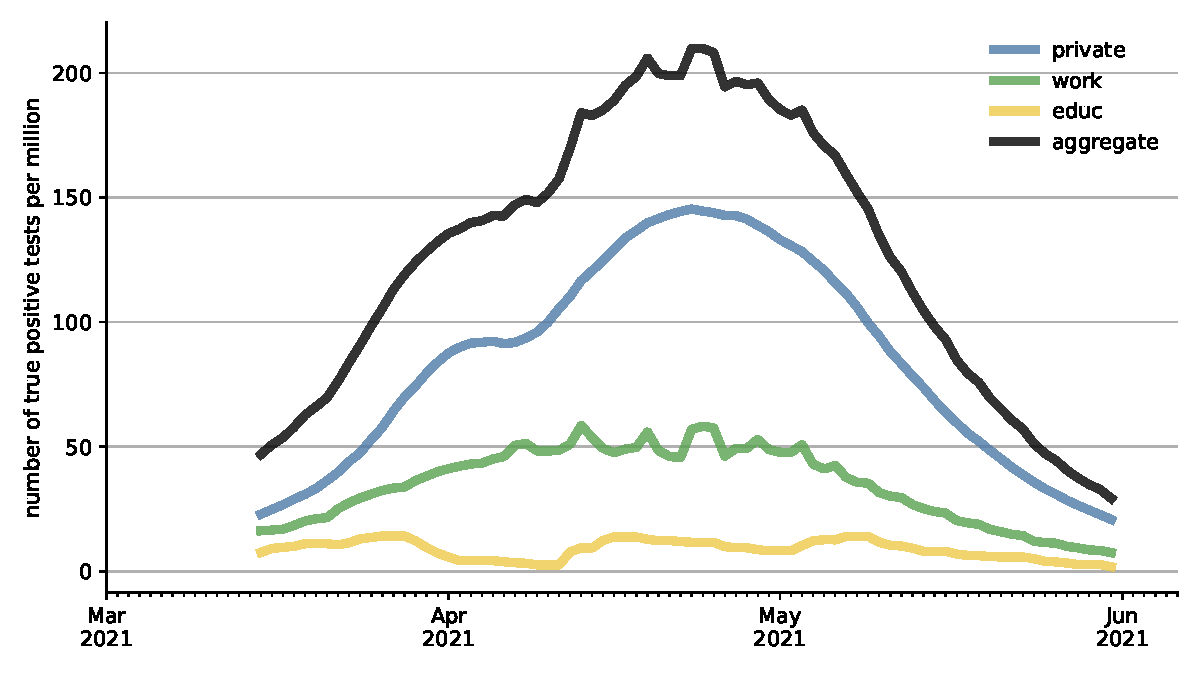
\includegraphics[width=\textwidth]{figures/results/figures/rapid_test_statistics/number_true_positive}
        \caption{Number of Discovered Cases Due to Rapid Tests by Channel}
        \label{fig:rapid_tests_number_true_positive}
    \end{subfigure}
    \hfill
    \begin{subfigure}[b]{0.425\textwidth}
        \centering
        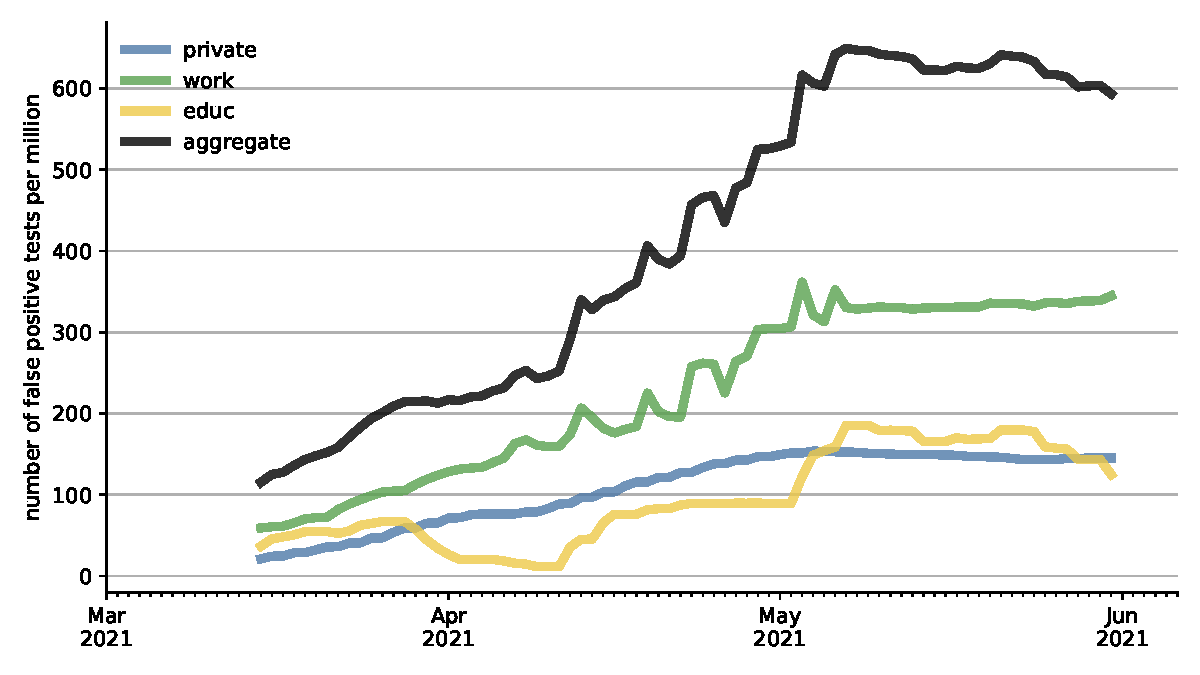
\includegraphics[width=\textwidth]{figures/results/figures/rapid_test_statistics/number_false_positive}
        \caption{Number of False Positive Rapid Tests by Channel}
        \label{fig:rapid_tests_number_false_positive}
    \end{subfigure}
    \vskip3ex
    \begin{subfigure}[b]{0.425\textwidth}
        \centering
        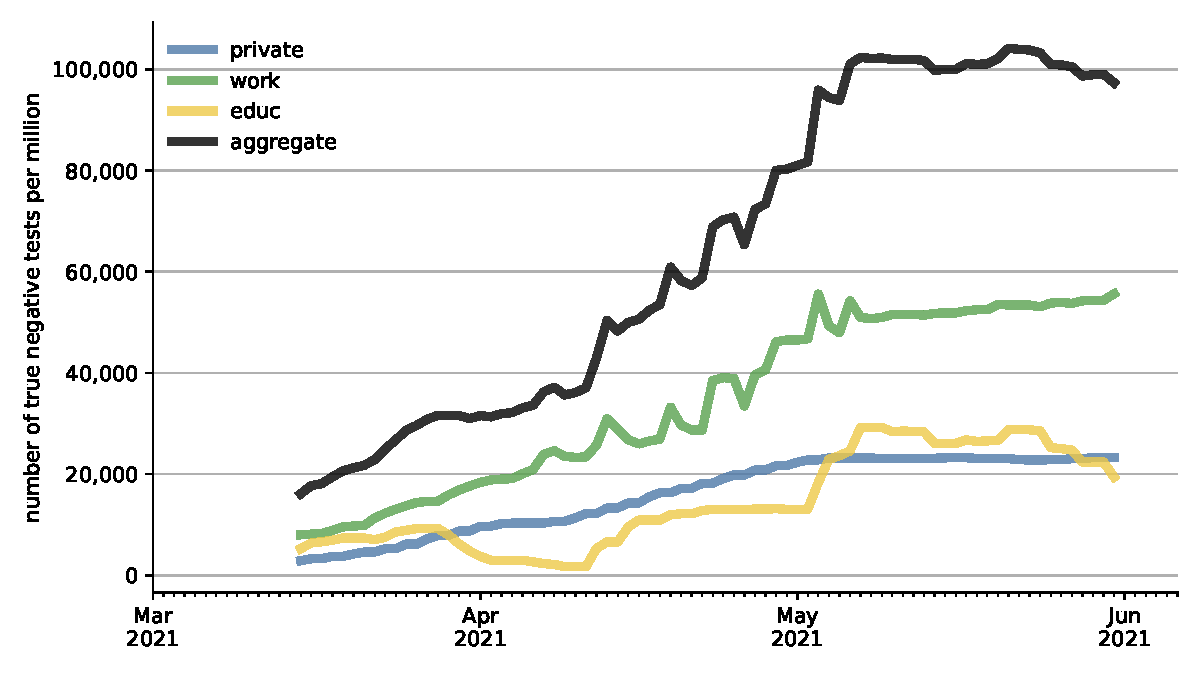
\includegraphics[width=\textwidth]{figures/results/figures/rapid_test_statistics/number_true_negative}
        \caption{Number of True Negative Rapid Tests by Channel}
        \label{fig:rapid_tests_number_true_negative}
    \end{subfigure}
    \hfill
    \begin{subfigure}[b]{0.425\textwidth}
        \centering
        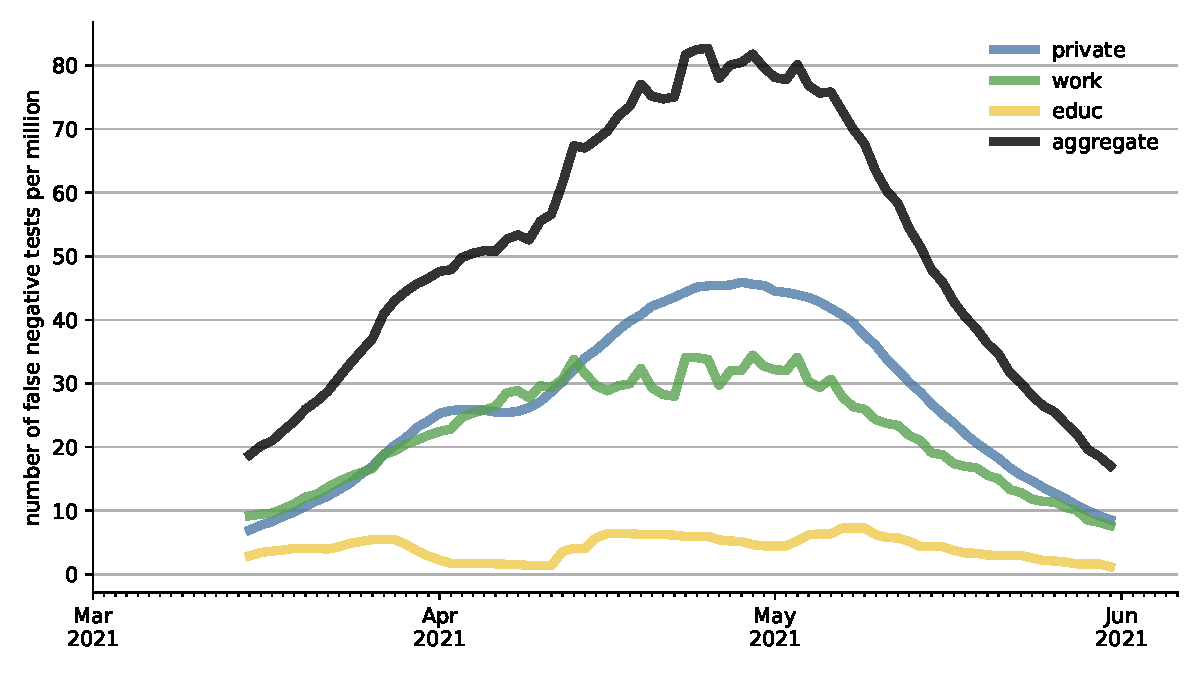
\includegraphics[width=\textwidth]{figures/results/figures/rapid_test_statistics/number_false_negative}
        \caption{Number of False Negative Rapid Tests by Channel}
        \label{fig:rapid_tests_number_false_negative}
    \end{subfigure}
    \vskip3ex
    \caption{Rapid Test Results}
    \label{fig:rapid_test_results_numbers}

    \floatfoot{\noindent \textit{Note:}
    Each panel shows the number of rapid tests per million inhabitants that fall into the
    respective category. Private rapid tests are especially good at detecting cases but
    since they are often triggered by rapid tests from other channels, the other groups
    of tests, especially rapid tests at the workplace, also play an important role for
    containing the pandemic. Since they are often triggered by rapid tests in the
    household private rapid tests are especially able to prevent infections because they
    are done soon after infection has taken place but are also more prone to return false
    negative results (see bottom right panel) because they are more likely to be
    performed before the onset of infectiousness.}
\end{figure}

\FloatBarrier

We now turn to the false positive and false negative rates, i.e. the share of positive
tests that go to people who are not truly infected and the share of negative tests that
go to individuals that are actually infected. The lower these numbers the more accurate
the test results. As can be seen in Figure~\ref{fig:rapid_tests_false_positive_rate} the
share of false positive rates is very high. On average 60\% to 93\% of positive tests are
received by individuals that are not infected. This is due to the low base rate, which
falls over time leading to an increase in the false positive rate. Again, private rapid
tests are an exception with a much lower false positive rate. Here the base rate of
individuals doing a rapid test through this channel is much higher because these tests
are often triggered by an event that makes it likely that the person doing the test is
actually infected. On the other hand, For the most part negative rapid tests are very
accurate with less than 0.2\% going to infected individuals at any point in time. One
exception are again the private rapid tests. Here, because they are triggered and are
thus performed very early, the chance of a false negative result is very high in the
beginning. As the incidences drop and less private rapid tests are triggered by positive
rapid tests in the household and a larger percentage of private rapid tests are done for
leisure activities, the false negative rate steeply decreases.

\begin{figure} % True Positive / False Positive / True Negative / False Negative Rate
    \centering
    % \begin{subfigure}[b]{0.425\textwidth}
    %     \centering
    %     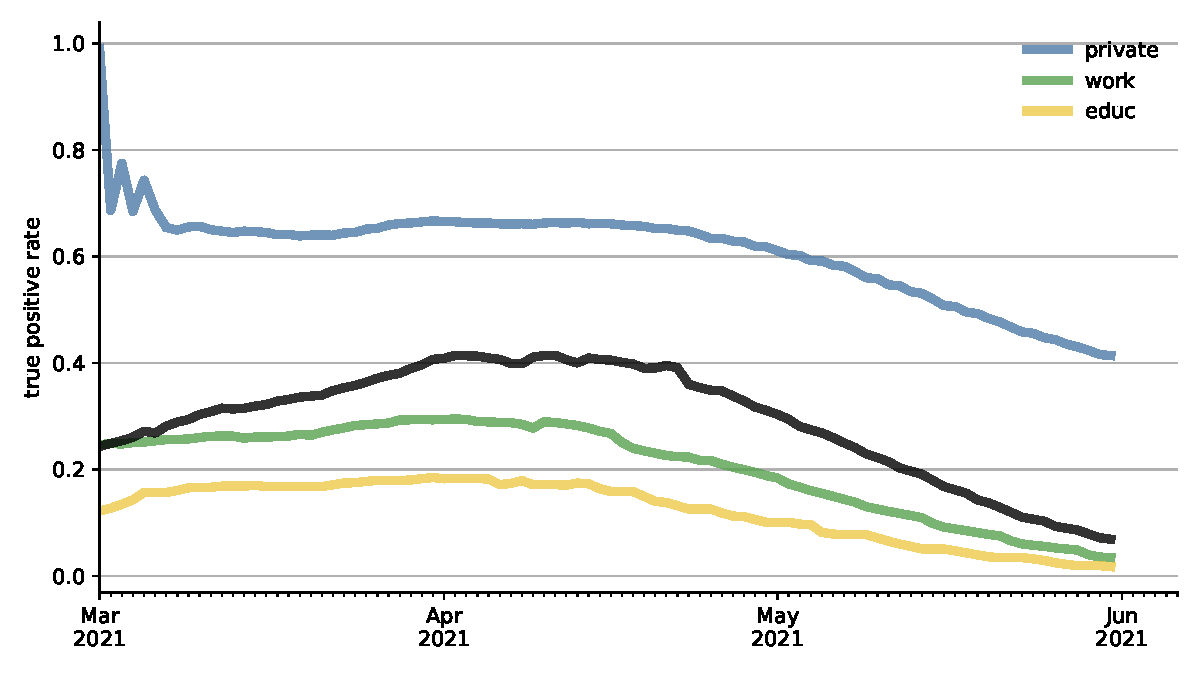
\includegraphics[width=\textwidth]{figures/results/figures/rapid_test_statistics/true_positive_rate}
    %     \caption{Rate of True Positive Rapid Tests by Channel}
    %     \label{fig:rapid_tests_true_positive_rate}
    % \end{subfigure}
    % \hfill
    \begin{subfigure}[b]{0.425\textwidth}
        \centering
        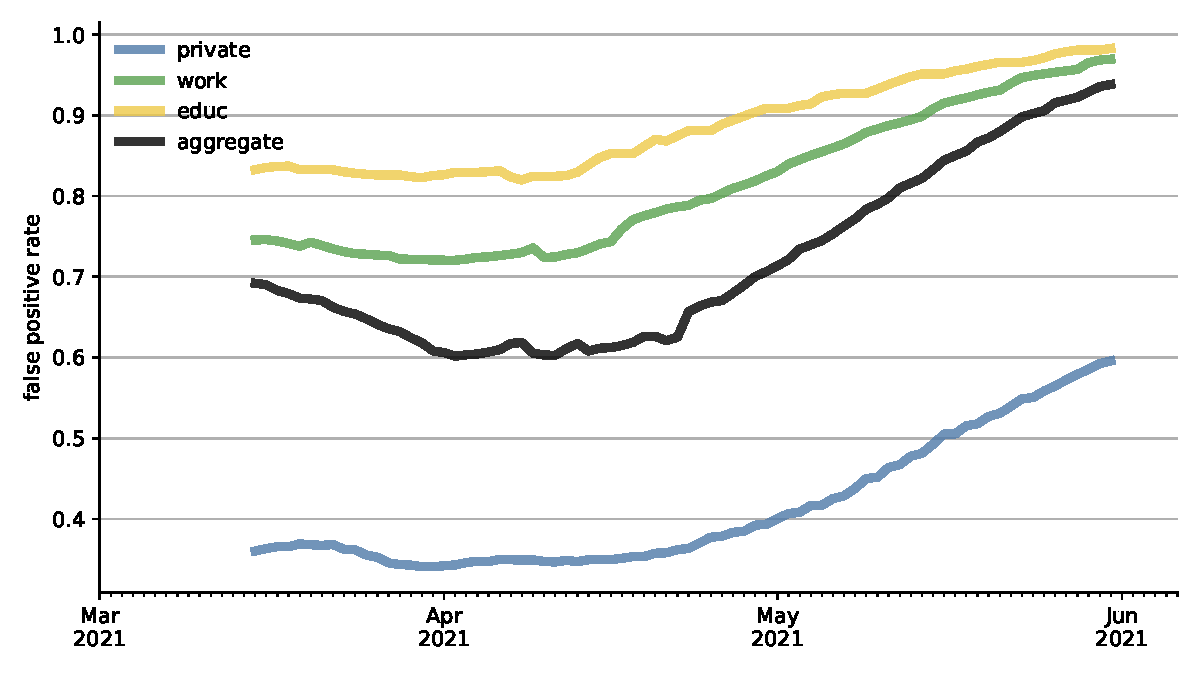
\includegraphics[width=\textwidth]{figures/results/figures/rapid_test_statistics/false_positive_rate}
        \caption{Rate of False Positive Rapid Tests by Channel}
        \label{fig:rapid_tests_false_positive_rate}
    \end{subfigure}
    % \vskip3ex
    % \begin{subfigure}[b]{0.425\textwidth}
    %     \centering
    %     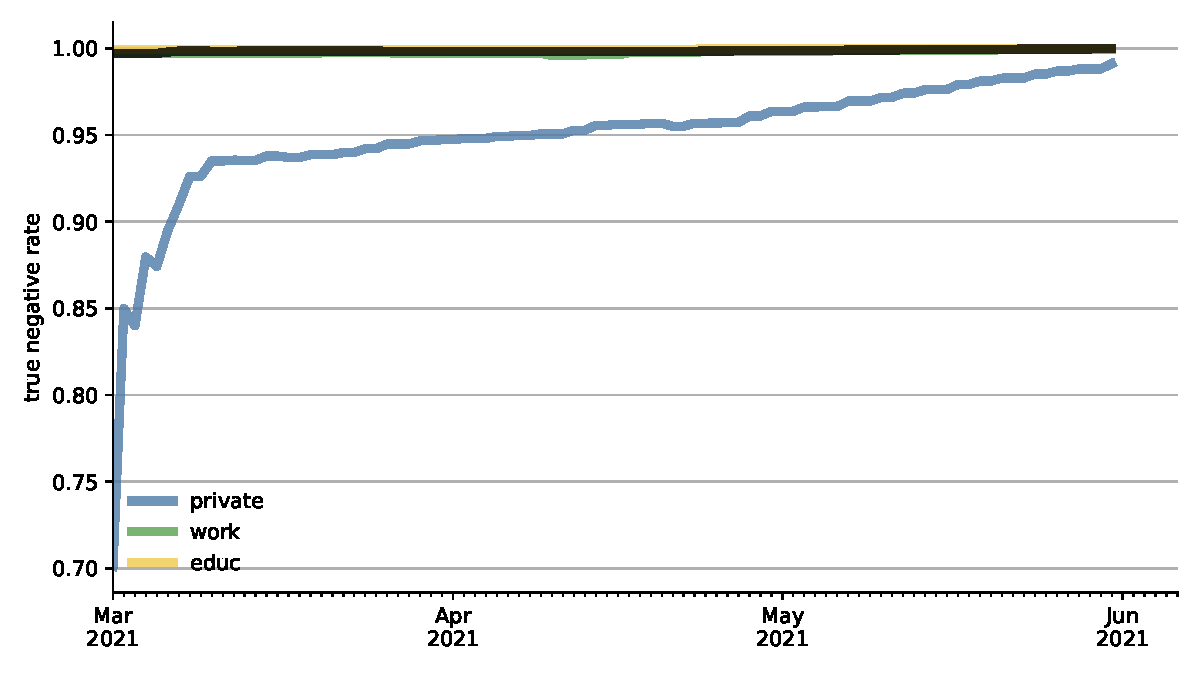
\includegraphics[width=\textwidth]{figures/results/figures/rapid_test_statistics/true_negative_rate}
    %     \caption{Rate of True Negative Rapid Tests by Channel}
    %     \label{fig:rapid_tests_true_negative_rate}
    % \end{subfigure}
    \hfill
    \begin{subfigure}[b]{0.425\textwidth}
        \centering
        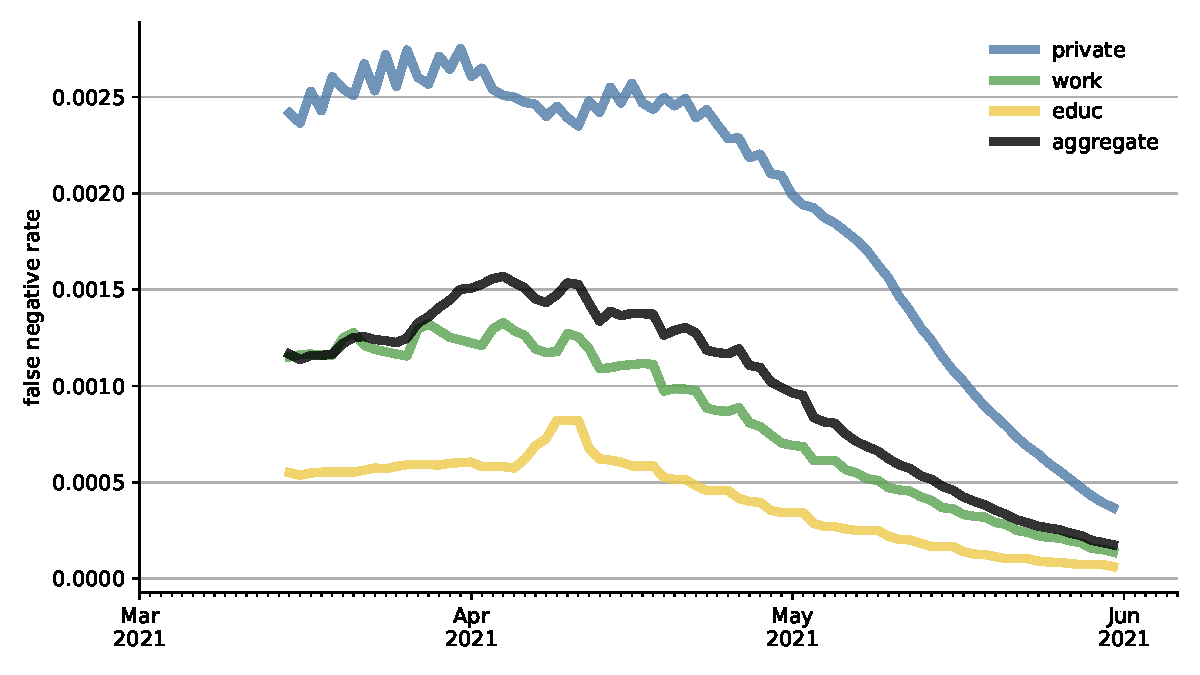
\includegraphics[width=\textwidth]{figures/results/figures/rapid_test_statistics/false_negative_rate}
        \caption{Rate of False Negative Rapid Tests by Channel}
        \label{fig:rapid_tests_false_negative_rate}
    \end{subfigure}
    \vskip3ex
    \caption{Rapid Test Rates by Channel}
    \label{fig:rapid_test_results_rates}

    \floatfoot{\noindent \textit{Note:}
    The left panel shows the share of positive tests that are given to people who are not
    infected. This share is large as can be expected with a very low baseline rate of
    positive individuals. As the incidence in the population drops, the false positive
    rate increases. An exception are the private rapid tests because they are --
    especially when the incidence is high -- often triggered by events that make it
    likely that the test taker is infected and therefore their false positive rate is
    much lower. The right panel shows the false negative rate in the population, i.e. the
    share of negative test results that are mistakenly given to infected individuals. Our
    simulations show that rapid tests are very good at detecting infected individuals
    overall. The only exception are private rapid tests because triggered rapid tests are
    likely to be performed early during an infection when the sensitivity of rapid tests
    is still rather low.
    }
\end{figure}

\FloatBarrier

 \comment[id=K]{@Janos: Please write the section on the testshares.}


\begin{figure} % Share of Tests That Are True Positive / False Positive / True Negative / False Negative
    \centering
    \begin{subfigure}[b]{0.425\textwidth}
        \centering
        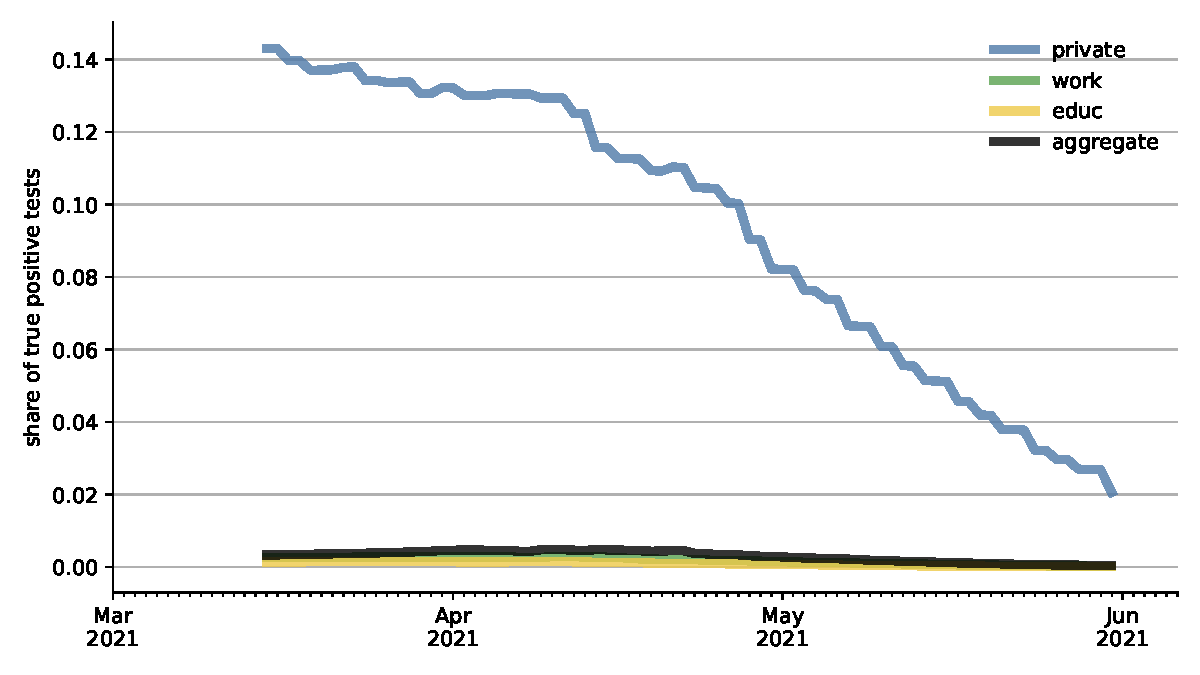
\includegraphics[width=\textwidth]{figures/results/figures/rapid_test_statistics/testshare_true_positive}
        \caption{Share of Tests That Are True Positive by Channel}
        \label{fig:rapid_tests_testshare_true_positive}
    \end{subfigure}
    \hfill
    \begin{subfigure}[b]{0.425\textwidth}
        \centering
        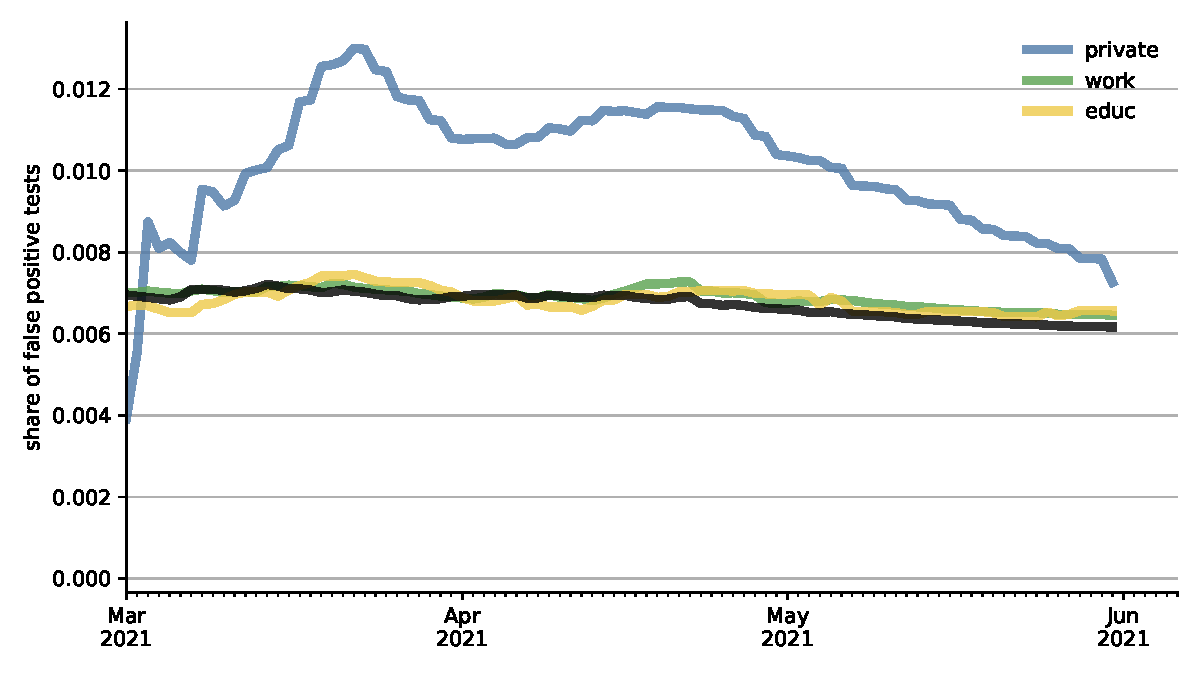
\includegraphics[width=\textwidth]{figures/results/figures/rapid_test_statistics/testshare_false_positive}
        \caption{Share of Tests That Are False Positive by Channel}
        \label{fig:rapid_tests_testshare_false_positive}
    \end{subfigure}
    \vskip3ex
    \begin{subfigure}[b]{0.425\textwidth}
        \centering
        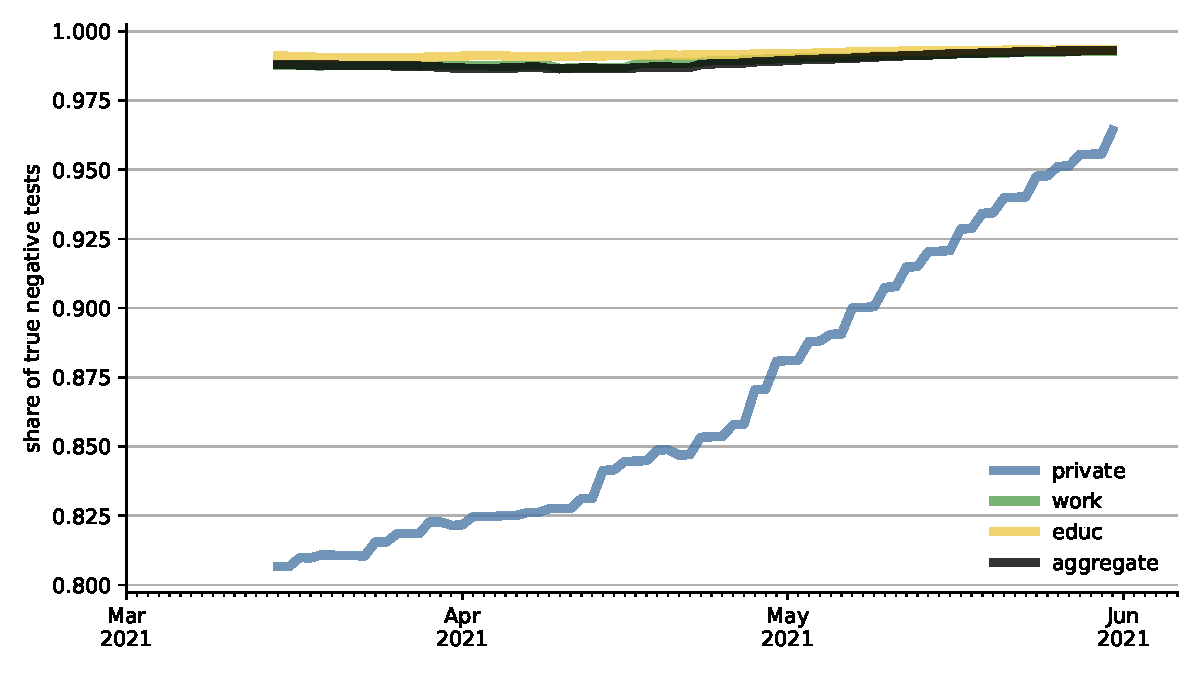
\includegraphics[width=\textwidth]{figures/results/figures/rapid_test_statistics/testshare_true_negative}
        \caption{Share of Tests That Are True Negative by Channel}
        \label{fig:rapid_tests_testshare_true_negative}
    \end{subfigure}
    \hfill
    \begin{subfigure}[b]{0.425\textwidth}
        \centering
        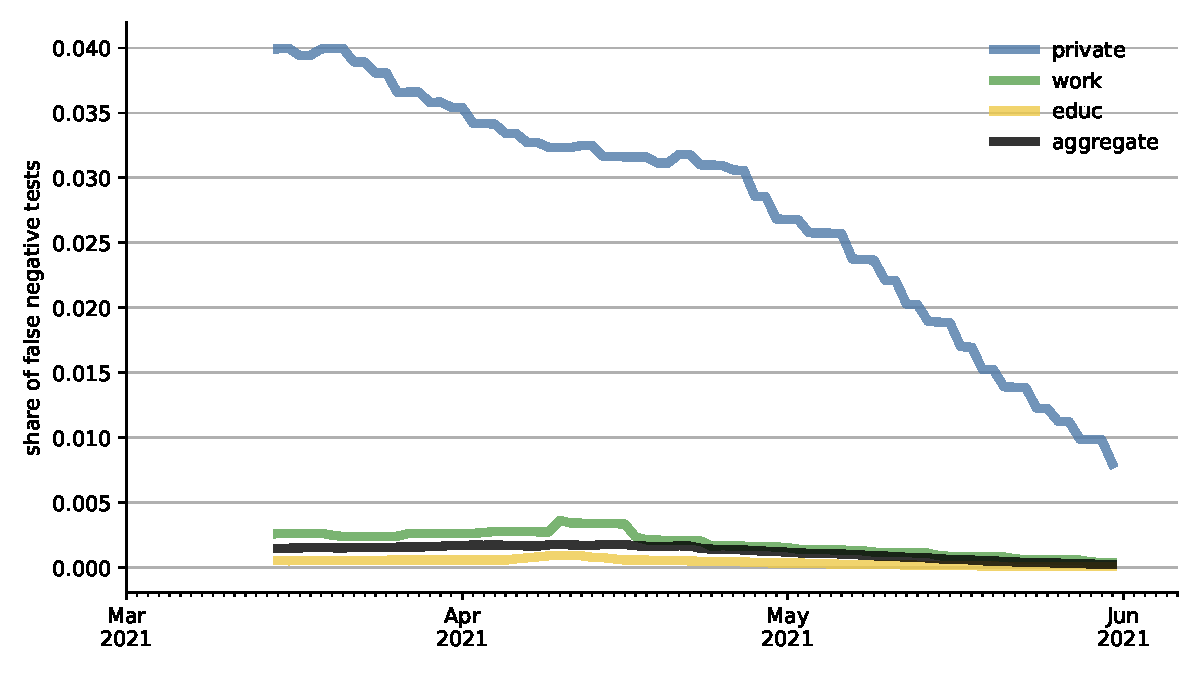
\includegraphics[width=\textwidth]{figures/results/figures/rapid_test_statistics/testshare_false_negative}
        \caption{Share of Tests That Are False Negative by Channel}
        \label{fig:rapid_tests_testshare_false_negative}
    \end{subfigure}
    \vskip3ex
    \caption{Share of Rapid Tests by Outcome and True Infection Status}
    \label{fig:rapid_test_results_test_shares}

    \floatfoot{\noindent \textit{Note:}
    This figure shows the share of all tests that are true positive, false positive, true
    negative and false negative. The share of true positives is very low, except for the
    targeted private rapid tests. The share of false positives is also very low, except
    for the private rapid tests that are more likely to be performed early during the
    infection when the sensitivity of rapid tests is still very low. Private tests also
    are the exception among the true negative results. Negative positive test results
    must be interpreted with caution when an individual is suspected to have been
    exposed, especially when that exposure has been recently as they are likely to return
    false negative results in the first few days of an infection. }
\end{figure}






\FloatBarrier